\renewcommand*{\arraystretch}{1.1}

\noindent\begin{tabularx}{\queryCardWidth}{|>{\queryPropertyCell}c|X|}
	\hline
	query & Interactive / update / 1 \\ \hline
%
	title & Add Person \\ \hline
%
    pattern & \hfill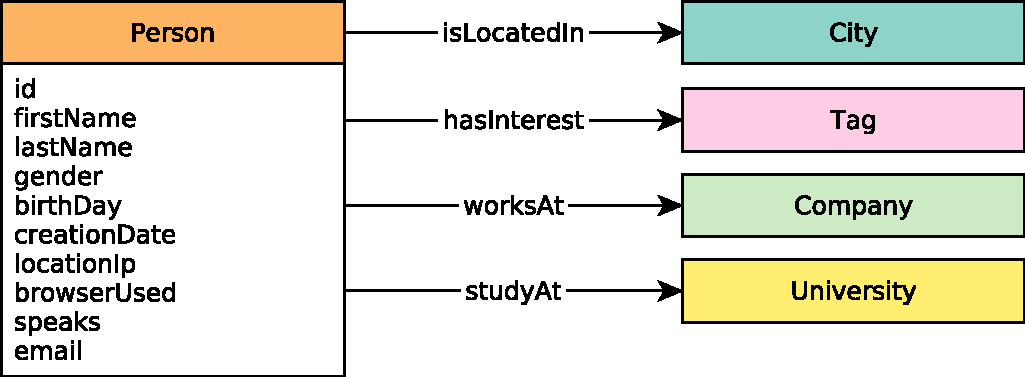
\includegraphics[scale=\patternscale,margin=0cm .2cm]{patterns/interactive-update-01}\hfill\vadjust{} \\ \hline
%
	desc. & Add a Person to the social network.
 \\ \hline
%
	
%
	params &
	\innerCardVSpace{\begin{tabularx}{\attributeCardWidth}{|>{\paramNumberCell}c|>{\varNameCell}M|>{\typeCell}m{\typeWidth}|Y|} \hline
	\cellcolor{parameter} \color{white} \footnotesize $\mathsf{1}$ &Person.id& ID &  \\ \hline
	\cellcolor{parameter} \color{white} \footnotesize $\mathsf{2}$ &Person.firstName& String &  \\ \hline
	\cellcolor{parameter} \color{white} \footnotesize $\mathsf{3}$ &Person.lastName& String &  \\ \hline
	\cellcolor{parameter} \color{white} \footnotesize $\mathsf{4}$ &Person.gender& String &  \\ \hline
	\cellcolor{parameter} \color{white} \footnotesize $\mathsf{5}$ &Person.birthDay& Date &  \\ \hline
	\cellcolor{parameter} \color{white} \footnotesize $\mathsf{6}$ &Person.creationDate& DateTime &  \\ \hline
	\cellcolor{parameter} \color{white} \footnotesize $\mathsf{7}$ &Person.locationIp& String &  \\ \hline
	\cellcolor{parameter} \color{white} \footnotesize $\mathsf{8}$ &Person.browserUsed& String &  \\ \hline
	\cellcolor{parameter} \color{white} \footnotesize $\mathsf{9}$ &Person-isLocatedIn->City.id& ID &  \\ \hline
	\cellcolor{parameter} \color{white} \footnotesize $\mathsf{10}$ &Person.speaks& \{String\} &  \\ \hline
	\cellcolor{parameter} \color{white} \footnotesize $\mathsf{11}$ &Person.email& \{String\} &  \\ \hline
	\cellcolor{parameter} \color{white} \footnotesize $\mathsf{12}$ &Person-hasInterest->Tag.id& \{ID\} &  \\ \hline
	\cellcolor{parameter} \color{white} \footnotesize $\mathsf{13}$ &\{Person-studyAt->University.id, Person-studyAt->.classYear\}& \{ID, 32-bit Integer\} &  \\ \hline
	\cellcolor{parameter} \color{white} \footnotesize $\mathsf{14}$ &\{Person-workAt->Company.id, Person-workAt->.workFrom\}& \{ID, 32-bit Integer\} &  \\ \hline
	\end{tabularx}}\innerCardVSpace \\ \hline
%
	
%
	%
	%
	%
    %
\end{tabularx}
\queryCardVSpace